\documentclass[journal, a4paper]{IEEEtran}
\usepackage{graphicx}
\usepackage{url}
\usepackage{amsmath}
\usepackage{amsfonts}
\usepackage{gensymb}


\begin{document}
	\title{Convolutional Pose Machines}
	\author{Clemens Pollak
	\thanks{Betreuer: M. Sc.~Bastian Wandt, Institut f\"ur Informations­verarbeitung, Leibniz Universit\"at, WS 2018/2019.}}
	\markboth{Seminar Computer Vision, Szenenanalyse und Codierung}{}
	\maketitle

%\begin{abstract}% TODO: abstract needed?
%\end{abstract}
\section{Einleitung}
	\IEEEPARstart{C}{onvolutional pose machines} sind neuronale Netze, welche die Pose von Menschen aus einem Bild extrahieren können. Mithilfe eines mehrstufigen Modells werden Schlüsselpunkte des Körpers detektiert. In dieser Seminararbeit wird beleuchtet, woher die Architektur und der Name kommen. Außerdem wird die Effektivität des Netzes untersucht und begründet.

        Diese Ausarbeitung beschäftigt sich zunächst mit der Fragestellung der Pose Estimation. Als erster Lösungsansatz werden Pose Machines von Ramakrishna et al.~\cite{ramakrishna2014pose} betrachtet. Der Kern der Arbeit ist die Untersuchung der Architektur von Convolutional Pose Machines~\cite{conv_pose} und den damit verbundenen Designentscheidungen.
        %TODO: when quotes?

\section{Pose estimation} \label{sec:pose_estimation}
	Eine Pose ist nach der DIN EN ISO 8373 (Industrieroboter Wörterbuch) eine Kombination von Position und Orientierung im dreidimensionalen Raum. In diesem Fall wird das Problem der Posen-Schätzung von Menschen in unterschiedlichen Bildern betrachtet. Das bedeutet: Die erkannten Posen werden zunächst nur zweidimensional erfasst. Im Bereich der Computer Vision werden Posen oft durch sogenannte Schlüsselpunkte dargestellt. Aus diesen Schlüsselpunkten kann man dann ein grobes Skelett zusammenfügen, dass die Pose des Menschen visualisieren kann (siehe Grafik~\ref{fig:hard_pose}).
        Für das Benchmark des MPII Datensatzes~\cite{MPII} 
        werden zum Beispiel folgende Schlüsselpunkte erwartet:
        \begin{itemize}
        \item Kopf 
        \item Nacken
        \item Rechte \& Linke Schulter
        \item Rechter \& Linker Ellenbogen
        \item Rechtes \& Linkes Handgelenk
        \item Brust
        \item Rechte \& Linke Hüfte
        \item Rechtes \& Linkes Knie
        \item Rechter \& Linker Knöchel
        \end{itemize}
        Zusammen mit dem Label für den Hintergrund gibt es in diesem Datensatz demzufolge 15 Label. In anderen Fällen können auch mehr Punkte nötig sein~\cite{lin2014microsoft}.
        \begin{figure}[!hbt]
                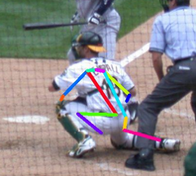
\includegraphics[width=0.4\columnwidth]{hardpose_1.png}
                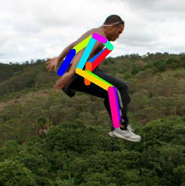
\includegraphics[width=0.35\columnwidth]{hardpose_2.png}
                \caption{Beispiele für schwierigen Posen aus~\cite{toshev2014deeppose}}
                \label{fig:hard_pose}
        \end{figure}
        In Grafik~\ref{fig:hard_pose} sieht man Beispiele, wo das erkennen von Schlüsselpunkten sehr schwierig ist. Einige Schlüsselpunkte, wie der Ellenbogen, sind überhaupt nicht sichtbar und können nur durch holistisches, logisches Denken erkannt werden.~\cite{toshev2014deeppose} Außerdem sind die Winkel aus denen Personen abgebildet sein können sehr unterschiedlich und die Gliedmaßen folgen keinen einfachen Anordnungsmustern.


\section{Pose Machines und andere Algorithmen zur Posen-Schätzung}
        Um die angesprochenen Probleme zu lösen, gibt es einige unterschiedliche Ansätze. %TODO: how much here?
        Die Idee der Convolutional Pose Machines~\cite{conv_pose} geht auf die Pose Machines~\cite{ramakrishna2014pose} zurück. Es handelt sich um eine Reihe von Klassifizierern, die von vorhergegangenen Fehlern lernen um immer bessere Schätzungen für Schlüsselpunkte zu erzeugen. 

        In der ersten Stufe produziert ein Klassifizierer\footnote{Wenn hier von Klassifizern gesprochen wird, dann handelt es sich immer um einen Multi-Klassen Klassifizierer, der für alle benötigten Schlüsselpositionen Schätzungen durchführen kann} initiale Schätzungen für die Position aller Schlüsselpunkte. Die Ausgabe sind sogenannte Belief Maps (siehe Grafik~\ref{fig:pose_machine}). Die Klassifizierer in den weiteren Stufen lernen die Belief Maps des vorigen Klassifizierer zu korrigieren, indem sie von vorigen Fehlern lernen. Idealerweise entstehen am Ende dann Belief Maps die klare Spitzen an den Stellen haben, die den Schlüsselpunkten im Originalbild entsprechen.

        \begin{figure}[!hbt]
                \begin{center}
                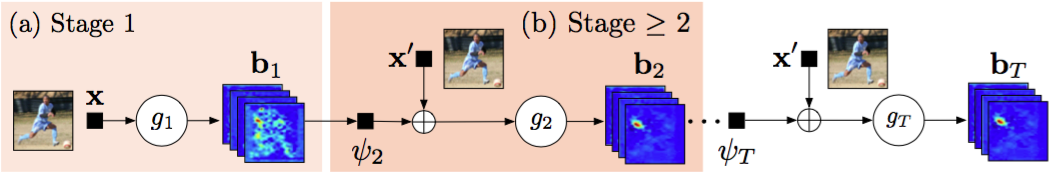
\includegraphics[width=1\columnwidth]{pose_machine.png}
                \caption{Pose Machine nach~\cite{ramakrishna2014pose}, aus~\cite{conv_pose}. Die beiden unterschiedlichen Architekturen der Stufen werden in Stufe Eins als $a)$ und Stufe Zwei bis $T$ als $b)$ unterteilt.}
                \label{fig:pose_machine}
                
                \end{center}
        \end{figure}

        Formal ist die Pose Machine definiert als eine Reihe von Klassifizierern $g_t$, wobei $g_1$ als eingabe nur das Eingabebild $x$ erhält. Jeder Klassifizierern erzeugt eine Matrix $b_{t}\in\mathbb{R}^{x*w*(P+1)}$. Dabei sind $h$ und $w$, Höhe und Breite des Bildes. P ist die Anzahl der Schlüsselpunkte. (P wird um Eins erhöht, weil der Hintergrund ebenfalls seperat erkannt wird)

        Die Ergebnisse $b_t$ dienen als Eingabe in die nächste Stufe. 
        Um die Informationen aus allen Belief Maps zu verarbeiten, wird auf $b_t$ eine Kontext-Merkmalfunktion $\psi_t$ angewendet. Diese verbindet "Context Patch Features" zum groben Erkennen der Konfidenz umliegender Schätzungen und "Context Offset Features" zum genauen Aufnehmen von relativen Postionsinformationen (das heißt relativ zu anderen Schätzungen). Die genaue Formel ist an dieser Stelle nicht zum Verstädnis relevant. %TODO: aber interessant?

        Die entstandene neue Belief Map wird dann mit dem Augangsbild addiert und bildet die Eingabe für den Klassifizierer der nächsten Stufe. In der finalen Stufe werden die Belief Maps dann auf Spitzen untersucht und anhand dessen die Positionen der Körperteile festgelegt.

        Zusammenfassend produziert der Klassifizierer $g_1$:
        \[ g_1(x_z) \rightarrow \{b_{1}^{p}(Y_p = z) \}_{p \in \{0 \ldots P\}} \] 
        Das bedeutet, dass aus Merkmalen des Bildes $x_z$ Belief Maps $b$ für jeden Schlüsselpunkt (und Hintergrund) erstellt werden. Diese Belief Maps bilden die geschätzte Wahrscheinlichkeit ab, das die jeweiligen Bildposition $Y_p \in Z$ der korrekten Schlüsselpunktpostion $z \in Z$ enspricht. Dabei sei $Z \subset \mathbb{R}_2$ die Gesamtheit aller möglichen Punkte im Bild.

        Wie zuvor beschrieben, produzieren die weiteren Klassifizerer $g_t$ eine Ausgabe mit gleichem Format und gleicher Bedeutung, erhalten aber zusätzlich zur Bildinformation $x_z$ noch die Ergebnisse der Kontext-Merkmalfunktion $\psi_t$:
        \[ g_t(x_z,\psi_t(z,b_{t-1})) \rightarrow \{b_{1}^{p}(Y_p = z) \}_{p \in \{0 \ldots P\}} \] 

        In der Arbeit von Ramakrishna et al.~\cite{ramakrishna2014pose} werden als Klassifizerer $g$ boosted random forests ~\cite{breiman2001,friedman2001greedy} gewählt. Zur Feature Extraction wird die Histogram of oriented Gradients (HoG) Methode~\cite{dalal2005histograms} verwendet.

\section{Convolutional Pose Machines}\label{subsec:Intro}
	In der Arbeit von Wei at al.~\cite{conv_pose} wird der Klassifizerer der Pose Machines durch eine "Deep Convolutional Architecture" ersetzt. Dadurch müssen keine Merkmale $x_z$ statisch aus dem Bild extrahiert werden und auch keine handgemachten Kontext-Merkmalfunktionen zum Einsatz kommen. Stattdessen ermöglicht es die Architektur, sowohl Merkmale des Kontext, als auch des Bildes selbst, direkt zu lernen. Außerdem können alle Stufen und damit alle Klassifizerer zusammen trainiert werden, weil die Architektur komplett differenzierbar ist. Bei Random Forests ist das nicht möglich~\cite{ramakrishna2014pose}.

        \begin{figure}[!bth]
                \begin{center}
                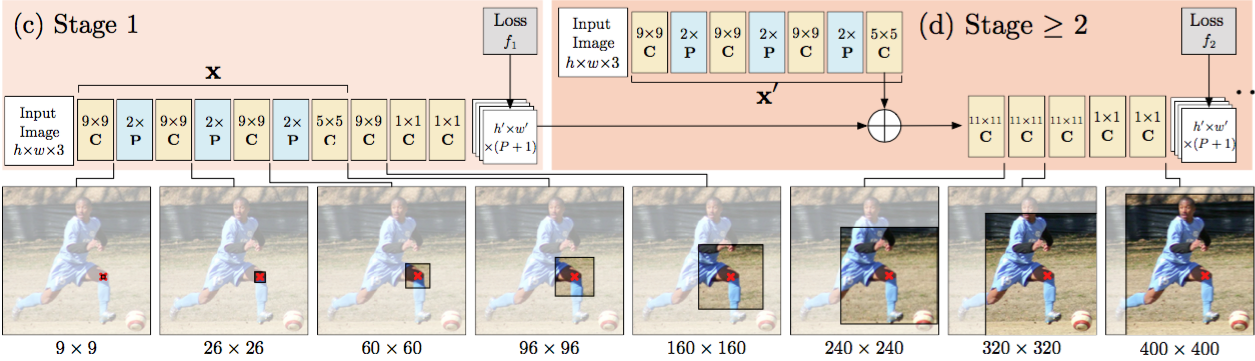
\includegraphics[width=1\columnwidth]{convolutional_pose_machine.png}
                \caption{Convolutional Pose Machine aus~\cite{conv_pose}. Die unterschiedlichen Architekturen der ersten und weiteren Stufen werden in Abschnitte $c)$ und $d)$ unterteilt. Im Abschnitt $e)$ wird das rezeptive Feld des Netzwerkes dargestellt. Es verdeutlicht wie viele räumliche Merkmale in die Schätzung einfließen.}
                \label{fig:conv_pose_machine}
                \end{center}
        \end{figure}

        In Grafik~\ref{fig:conv_pose_machine} sieht man die Architektur der Convolutional Pose Machines. Insbesondere kann man sehen, dass die Merkmalextrahierung durch Convolutional Layer und Pooling Layer ersetzt wurde. Dabei wird in der ersten Stufe eine andere Struktur zur Extrahierung verwendet als bei den folgenden Stufe. (siehe Grafik~\ref{fig:conv_pose_machine}, Teil $d$, Markierung $x'$) Bei einfachen Pose Machines bleibt die Extrahierung immer gleich. 

        In der ersten Stufe werden nach den Layern, die die Extrahierung ersetzen noch drei weitere Convolutional Layer angehängt, die anstelle des Klassifizierers stehen. Zusammen kann dieses Faltungsnetzwerk eine Belief Map erstellen, indem die Funktion der Feature Extrahierung und des Belief Mapping antrainiert wird. Dazu befindet sich nach jeder Stufe eine Verlustfunktion $f_{t}$.

        Die Verlustfunktion bestraft einen großen euklidischen Abstand zwischen den geschätzten und idealen Belief Maps. Dabei ist eine ideale Belief Map $b_{*}^{p}(Y_p = z)$. Sie entsteht durch das Überlagern mit Gaußfunktionen an den Stellen, wo sich die Schlüsselpunkte im Ground Truth befinden. %TODO: was ist mit dem Hintergrund?
        Die zu minimierende Verlustfunktion in jeder Stufe ist deshalb gegeben durch:
        \[ f_t = \sum_{p=1}^{P+1} \sum_{z \in Z} ||b_{t}^{p}(z) - b_{*}^{p}(z) ||_{2}^{2}\]
        Da diese Verlustfunktion nach jeder Stufe angewendet wird, entstehen nach jeder Stufe interpretierbare Belief Maps. Außerdem helfen die Verlustfunktionen beim Trainieren des Netzwerkes (siehe Abschnitt~\ref{subsec:vanishing_gradients}). Für das Ende-zu-Ende Training des Netzwerkes werden einfach alle Verlustfunktionen addiert:
        \[ F = \sum_{t=1}^{T} f_t \]


        Die Kontext-Merkmalfunktion $\psi_t$ fällt bei den Convolutional Pose Machines weg, da auch dieses Verhalten antrainiert werden kann (siehe Abschnitt~\ref{subsec:kontext}). Deshalb wird die Belief Map direkt mit dem Ergebnis der Merkmalextrahierung $x'$ addiert und mit 5 weiteren Convolutional Layern zu einer neuen Belief Map verarbeitet. 

\subsection{Merkmale im Kontext}\label{subsec:kontext}
        Wie in den Pose Machines ist das Ziel der Convolutional Pose Machines, lokale Merkmale mit Umgebungsmerkmalen zu Verbinden. Die neue Architektur kann Vorteile von Deep Learning Methoden~\cite{toshev2014deeppose} und Graph basierten Methoden~\cite{andriluka2009pictorial,LanWM11} verbinden. %TODO: fraglich
        In Grafik~\ref{fig:conv_pose_machine}, Abschnitt $e)$ sieht man, dass das rezeptive Feld des Netzwerkes durch die Faltungen wächst. So werden mehr und mehr Merkmale einbezogen, die nicht in unmittelbarer Nähe des untersuchten Punktes sind. Diese Aufgabe hatte bei den Pose Machines die handgemachte Funktion $\psi$. Im Idealfall kombiniert das Netzwerk die Informationen über Vorhersagen von anderen Schlüsselpunkten und Merkmalextrahierung besser als $\psi$ zuvor.

        Das rezeptive Feld eines Convolutional Neural Networks ist der Bereich auf dem Ausgangsbild, der Einfluss auf die Ausgabe des jeweiligen Layers hat. Dabei nimmt der Einfluss vom Zentrum zu den Randbereichen exponentiell ab~\cite{dumoulin2016guide}. 
        Die Größe des Feldes kann mit folgender Formel berechnet werden~\cite{dumoulin2016guide}:
        \[ r_{out} = r_{in} + (kernel-1) * d_{in}\]
        \[ d_{out} = d_{in} * stride\]
        Dabei ist $r$ das rezeptive Feld, und $d$ die Distanz zwischen zwei Merkmalen. $stride$ ist die Schrittweite und $kernel$ ist die Kernelgröße der Convolution im jeweiligen Layer. Die Feldgröße kann so rekursiv für alle Layer berechnet werden.
        

        Ein größeres rezeptives Feld kann folglich durch unterschiedliche Anpassungen erreicht werden. Es können Pooling Operationen ausgeführt werden, die Kernelgröße oder Schrittweite kann erhöht werden, oder es werden mehr Convolutional Layer hinzugefügt.
        Die Autoren nutzen die Pooling Layer nur zur Feature Extraction, weil bei Pooling Operationen immer Daten verworfen werden. Dies führt gegebenfalls zu niedrigerer Genauigkeit. Deshalb nennt sich das Netzwerk auch Fully Convolutional. Man könnte die Größe des Feldes auch durch einen größeren Faltungskernel vergrößern. Ein größerer Kernel erhöht allerdings die Anzahl der Parameter im Netzwerk und verlangsamt es. 
        Aus diesem Grund haben sich die Autoren für eine Architektur mit vielen Convolutional Layer entschieden. Eine höhere Anzahl von Layern kann ihrerseits das Vanishing Gradient Problem hervorrufen. Da das Vanishing Gradient Problem durch mehrere Verlustfunktionen abgefedert werden kann (siehe Abschnitt~\ref{subsec:vanishing_gradients}), ist dies jedoch das geringste Übel. Die Belief Maps werden werden trotzdem nach jeder Stufe um einen Faktor 8 herunterskaliert, um weniger Parameter im Netzwerk zu benötigen. Die Schrittweite der Faltungen haben die Autoren experimentell festgelegt. Es hat sich eine Schrittweite von 8 bewährt. Die Parameteranzahl wird weiterhin durch geteilte Gewichte reduziert. Weil alle Stufen, außer der Ersten, die gleiche Funktion übernehmen, können die Gewichte von korrespondierenden Faltungen der Layer geteilt werden.

        \begin{figure}[!hbt]
                \begin{center}
                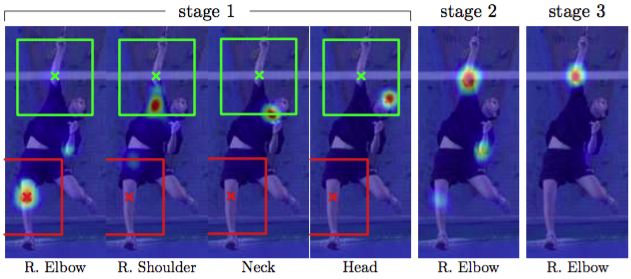
\includegraphics[width=1\columnwidth]{receptive_field.png}
                \caption{Belief Maps einer drei Stufen Convolutional Pose Machine. Eingeblendet sind zwei rezeptive Felder des kompletten Netzwerkes mit einer Größe von 160x160 Pixeln. In Rot sieht man das Feld zentriert auf der ersten Schätzung für den rechten Ellenbogen. In Grün sieht man das Feld zentriert auf der Stelle des Ellenbogen vom Ground Truth. Es ist zu sehen, dass die schlechte Schätzung der ersten Stufe korrigiert wurde.}
                \label{fig:receptive_field}
                \end{center}
        \end{figure}

        Wie in Sektion~\ref{sec:pose_estimation} erläutert, sind Schlüsselpunkte, die weit vom Rumpf entfernt sind, schwer zu erkennen. 
        In Grafik~\ref{fig:receptive_field} sieht man, dass das rezeptive Feld andere Peaks in den Belief Maps einschließt. Dadurch kann die Information über die Morphologie des Köpers genutzt werden, um schlechte Schätzungen zu korrigieren. In diesem Fall könnte zum Beispiel die korrekte Erkennung von Kopf, Schulter und Nacken dazu beigetragen haben, die Position des Ellenbogens in der zweiten Stufe zu verschieben. Man kann außerdem beobachten, dass der Peak, welcher sich an der falschen Stelle befindet, deutlich breiter ist als andere. Dies kann eine "Unsicherheit" in der Schätzung bedeuten.

        Diese qualitativen Beobachtungen wurden durch Experimente bestätigt, indem das rezeptive Feld bei gleicher Parameteranzahl vergrößert wurde. Es kam zu einer signifikanten Verbesserung der Genauigkeit~\cite{conv_pose}.
        %TODO: more here?

\begin{figure*}
        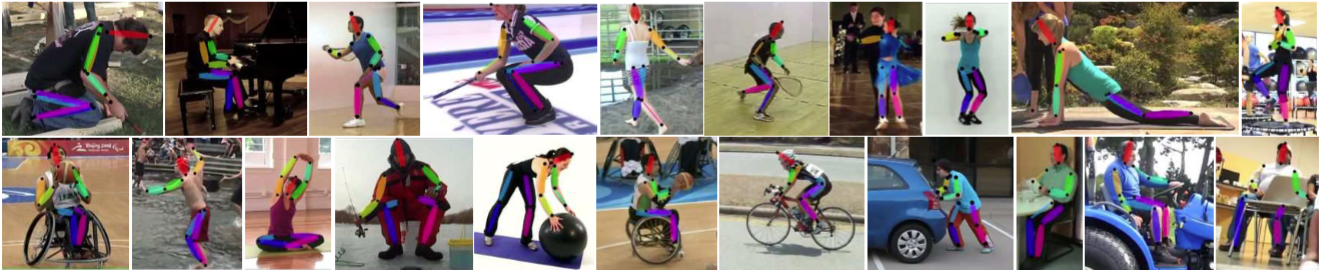
\includegraphics[width=2\columnwidth]{mpii_results.png}
        \caption{Qualitative Resultate auf dem MPII Datensatz. Man kann beobachten, dass die Schlüsselpunkte für unterschiedliche Posen und Winkel erkannt werden.}
        \label{fig:mpii_results}
\end{figure*}
\begin{figure*}
        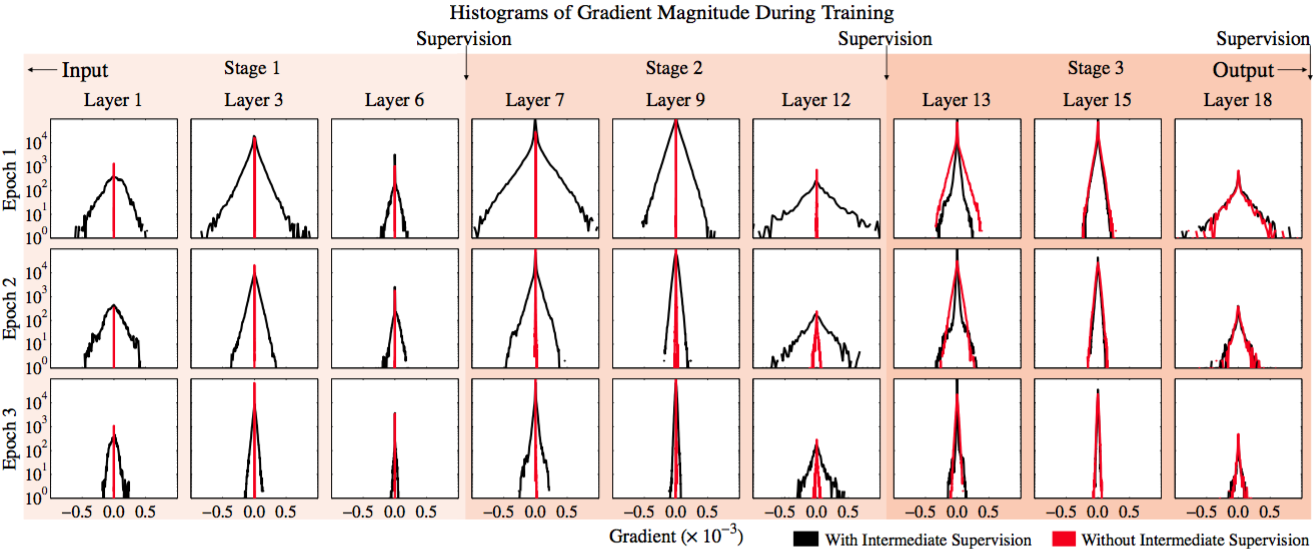
\includegraphics[width=2\columnwidth]{intermediate_supervision.png}
        \caption{In den Histogrammen wird die Größe der Gradienten über drei Epochen des Trainings abgebildet.}
        \label{fig:intermediate_supervision}
\end{figure*}

\subsection{Training und Vanishing Gradients} \label{subsec:vanishing_gradients}

        Die Architektur einer Convolutional Pose Machine kann viele Convolutional Layer enthalten. Diese Tiefe ist ein Problem, denn es können sogenannte Vanishing Gradients auftreten~\cite{pascanu2013difficulty}. Das heißt, dass bei der Back-Propagation die Gradienten der Layer zwischen Ein- und Ausgabe immer kleiner werden und praktisch "verschwinden". Ein effizientes Training ist dann nicht mehr möglich.

        Durch die Architektur der Pose Machines kann die Anzahl der Layer zwischen Input und Output jedoch reduziert werden. Dazu dienen die Verlustfunktionen nach jeder Stufe. Sie erzwingen die Ausgabe der Belief Maps und sorgen damit dafür, dass auch in den Layern der mitteleren Stufen Ergebnisse erzeugt werden und die Gradienten nicht verschwinden. Im folgenden wird diese Taktik Intermediate Supervision genannt.

        Das Problem der Vanishing Gradients kann auch experimentell gezeigt werden. In Grafik~\ref{fig:intermediate_supervision} kann man Gradienten von 9 beispielhaft ausgewählten Layern sehen und deren Veränderung über drei Epochen des Trainings. In Schwarz ist die normale Architektur und in Rot eine Trainingslauf ohne Intermediate Supervision dargestellt. Man kann deutlich erkennen, dass die Varianz der Gradienten im Fall ohne Intermediate Supervision sehr klein ist. Die Gradienten bewegen sich um Null. Das heißt: Die Neuronen dieser Layer werden wenig Informationen weitergeben und tragen wenig zur Klassifizierung bei. Veränderungen finden hautpsächlich in den letzten Layern statt. Im Fall mit Intermediate Supervision ist die Varianz deutlich größer und scheint nur langsam über die Epochen zu sinken. Das gilt für alle dargestellten Layer, auch jene welche nicht direkt vor einer Verlustfunktion stehen. Die intermediate supervsion scheint folglich in einem guten Abstand eingesetzt zu sein.

\subsection{Die beste Konfiguration}
        
        Nach den bereits diskutierten Designentscheidungen wurde die Anzahl der Stufen experimentell optimiert. Bei Tests auf dem Leeds Sports Pose Dataset\footnote{mit person centric annotations (PC)}~\cite{LSP} ergab sich, dass mehr Stufen grundsätzlich eine höhere Genauigkeit ergeben. Allerdings verbessert sich die Genauigkeit immer geringer, je mehr Stufen es gibt. Die Autoren haben sich entschieden eine 6 stufige Architektur zu evaluieren. Sie benutzen normalisierte Eingabebilder mit der Größe 368x368 Pixel. Dabei werden die Ursprungsbilder zuerst skaliert und anhand von Größe und Schlüsselpunkten zugeschnitten oder gepaddet. Es wurden außerdem unterschiedliche Trainingsmethoden getestet, wobei sich das Ende-zu-Ende Training als bestes heraustellte.

\section{Evaluation}

        Diese Seminararbeit beschränkt sich auf die Evaluation mit dem prominentesten Datensatz, das MPII Humand Pose Dataset~\cite{MPII}. Der Datensatz besteht aus mehr als 28000 Trainingsbildern. Für das Training wurden die Daten Augmentiert. Dabei wurden zufällig Rotationswinkel [-40\degree,40\degree], Skalierungsfaktoren [0.7,1.3] und horizontales Spiegeln verwendet. Als Metrik wird die PCKh Metrik verwendet. %TODO: was ist das? - cite
        Weil in diesem Datensatz auch mehrere Personen auf einem Bild sichtbar sein können, wurden zwei Sets von Belief Maps für das Training erstellt. Eine enthält alle Peaks für jede Person in der Nähe der Hauptperson. Die Zweite enthält nur Peaks für die Schlüsselpunkte der Hauptperson.
        Die erste Art von Belief Maps wird für die Verlustfunktion der ersten Stufe verwendet, weil hier nur lokale Zusammenhänge erlernt werden. In allen weiteren Stufen wird das zweite Set verwendet, um geometritsche Relationen zwischen den Peaks richtig abzubilden.

        Das Ergebnis nach der PCKh-0.5 Metrik war zur Zeit der Veröffentlichung State of the Art mit einer Detektionsrate von 88.0\%. Wenn zusätzlich noch der Leeds Sport Pose Datensatz zum Training benutzt wurde, kam das Netzwerk auf ein Ergebnis von 88.5\%. 2016 war dieses Ergebnis mehr als 6\% besser als vergleichbare Methoden. Zur Zeit dieser Seminararbeit befindet sich die Convolutional Pose Machine auf Platz 12 in der offiziellen Rangliste~\cite{MPII}. State of the Art ist Tang et al.~\cite{tang2018deeply} mit einer Wertung von 92.3\%
        
\section{Fazit und aktuelle Arbeiten}
        Die Convolutional Pose Machines entstanden aus der Kombination von neuen Deep Learning Techniken und der Idee, Kontext über ein Stufenmodell erlernen zu lassen. Die Autoren haben im Jahr 2017 ein bedeutendes Paper im Bereich des Multiple People Tracking veröffentlicht, das die hier dargestellten Ansätze weiter verfolgt~\cite{cao2017realtime,wei2016cpm}. Die Ideen der Intermediate Supervision sind immer noch relevant. Allerdings gibt es auch Methoden, wie zum Beispiel Batch Normalization, die nicht im Paper über Convolutional Pose Machines betrachtet wurden. Da sich das Feld des Maschinellen Lernens sehr schnell bewegt, sind die Ergebnisse zwar deutlich überboten worden, aber trotzdem von Bedeutung.


\bibliographystyle{IEEEtran}
\bibliography{ausarbeitung}

\end{document}